\documentclass[12pt, aspectratio=43]{beamer}

\usepackage{pablo}

\begin{document}

\begin{frame}
  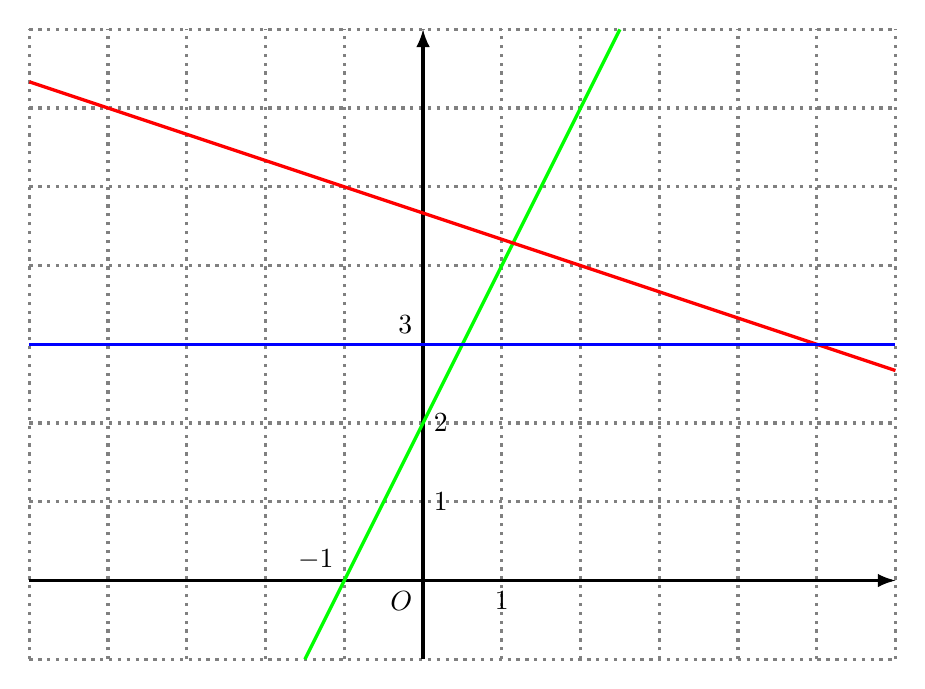
\begin{tikzpicture}[very thick,xscale=1, yscale=1]
    \draw[dotted, gray, xstep=1, ystep=1] (-5, -1) grid (6, 7);
    \draw[-latex] (-5,0) -- (6,0);
    \draw[-latex] (0,-1) -- (0,7);
    \draw (0,0) node[below left]{$O$};
    \draw (-1,0) node[above left]{$-1$};
    \draw (1,0) node[below]{$1$};
    \draw (0,1) node[right]{$1$};
    \draw (0,2) node[right]{$2$};
    \draw (0,3) node[above left]{$3$};

    \draw[green] (-1.5, -1) -- (2.5, 7);
    \draw[red] (-5, {19/3}) -- (6, {8/3});
    \draw[blue] (-5, 3) -- (6, 3);


  \end{tikzpicture}

\end{frame}
\end{document}
